\section{Modelación y diseño}
\label{sec:design}
El primer paso consiste en definir qué método utilizar para obtener una representación de la música (sobreponiéndose a la brecha semántica), que pueda ser utilizada para la recuperación semántica con consultas textuales.

Una de las estrategias de recuperación de información (con consultas textuales) utilizada extensamente, como se ha mencionado anteriormente, es mediante metadatos. Pero también hemos de recordar que dicha estrategia requiere que las canciones contengan metadatos curados (que no es muy práctico en los escenarios actuales donde la multimedia se genera en grandes cantidades, y libremente). Además, como segunda desventaja, la información conocida sobre las canciones estaría limitada al conjunto fijo de metadatos que se predefinan. 

Si se extraen los metadatos (tags, features) automáticamente con modelos de Machine Learning de clasificación y auto-tagging, se hace frente al primer problema mencionado: como hacer que todas las canciones tengan metadatos, sin requerir una cantidad de trabajo humano irrealista. Dado que los tags se extraen automáticamente, se abre una ventana a contrarrestar la segunda desventaja, ya que la cantidad de tags dependería de la cantidad de modelos de Machine Learning. Esto incluso permite que el conjunto no sea fijo. Con el costo de reprocesar la base de datos, se hace posible actualizar y añadir valores.

Otra estrategia, que ha sido analizada por las escasas investigaciones en el tema, es diseñar un modelo para convertir la música al espacio del lenguage natural, o convertir las descripciones textuales y la música a un espacio compartido. El problema fundamental de este acercamiento es que requiere un conjunto bastante grande de pares texto-audio, con suficiente diversidad y abarcamiento para maximimar la generalización del modelo. La inexistencia de dichos \textit{datasets} \cite{Simonetta2019MultimodalMI, Huang2022MuLanAJ, Manco2022ContrastiveAL}, en conjunto con la dificultades de requerimientos computacionales; no nos permiten realizar el entrenamiento necesario para implementar esta estrategia. 

Nuestra propuesta, extraer los features automáticamente, trabaja bajo la premisa de que el campo de MIR se ha desarrollado en tareas de clasificación y auto-tagging lo suficiente para ser competitivo con metadatos hechos a mano; relativo al esfuerzo que conlleva cada uno. % TODO specify a little more on our proposal

Para garantizar que el sistema de recuperación tenga en cuenta la similitud semántica, se propone utilizar un aceramiento con \textit{Sentence BERT} \ref{subsec:semantic_embedd} para comparar las consultas con las descripciones de la música. Los acercamientos tradicionales en SRI para mantener la significación semántica, suelen requerir estructuras complejas y un largo tiempo de pre-procesamiento o de ranking (como Latent Semantic Analysis (LSA) \cite{Foltz1996LatentSA}) . Con el auge de los modelos de lenguaje (alrededor de los últimos de cinco años) y su capacidad de capturar significado semántico y relación contextual; se ha abierto el camino para combinar la eficiencia del modelo vectorial con bolsa de palabras y el aumento en precisión de los modelos como LSA. 
% TODO explain the relationship between language models and the combination 

Dado que SBERT captura el embedding de un texto, y que el framework de extracción de features lo que devuelve es una lista de tags, es necesario convertirla a texto en lenguaje natural.  

La tarea de generación de texto a partir de tablas (\textit{table-to-text generation}) consiste en tomar una tabla estructurada como entrada y producir una descripción en lenguaje natural \cite{Yang2021TableTT}. Tiene buenas perspectivas de aplicación en la comunicación con humanos de manera comprensible y natural, como en la generación de informes financieros, informes médicos, etc. 

Efectivamente la mejor alternativa que se encontró para convertir los features en texto fue \textit{TableGPT: few-shot Table-to-text generation with Table Structure Reconstruction and Content Matching}. TableGPT \cite{Gong2020TableGPTFT} se enfoca en generar texto de alta fidelidad para la generación de texto a partir de tablas con un número limitado de pares de entrenamiento. Abordando la brecha entre la entrada de tablas estructuradas y la entrada de lenguaje natural que procesa GPT-2 durante el pre-entrenamiento, TableGPT intenta transformar naturalmente las tablas estructuradas en lenguaje natural. Sin embargo este modelo no se encuentra accesible para ser utilizado directamente con inferencia. Para utilizarlo sería necesario recrear todo su proceso de entrenamiento. Pero en el desarrollo de la investigación no se contó con los recursos computacionales para efectuarlo.

Entonces las propuestas factibles son: 
\begin{itemize}
    \item utilizar GPT-2 para generar descripciones a partir de la lista de metadatos
    \item crear una oración con fuerza bruta, por ejemplo para el género: `` The music genre sounds like \{\textit{genre classification}\}. ''
    \item utilizar un aceramiento similar a \cite{Manco2022ContrastiveAL} de concatenar tags en un oración
\end{itemize}
La primera requiere hacer \textit{prompt engineering} y no garantiza fidelidad con los datos extraídos. Mientras que las otras dos resultarían en descripciones que distan de la forma en que las personas realmente realizan consultas. 

Teniendo en cuenta todo esto, se propone intentar las tres estrategias de convertir tags en descripciones y comparar los resultados con las tres alternativas.\\

En conclusión, para la implementación del prototipo objetivo; que consiste en una plataforma donde realizar consultas en lenguaje natural sobre una base de datos de música y obtener resultados con significación semántica; la propuesta (como se puede observar en la imagen \ref{fig:corpus_embeddings}) consiste en:

\begin{itemize}
    \item un sistema de extracción de features compuesto por modelos de clasificación de música (incluyendo features de bajo y alto nivel).
    \item las características extraídas, entonces, son convertidas en descripciones utilizando las tres alternativas mencionadas anteriormente, obteniendo tres corpus de \textit{captions}.
    \item finalmente las descripciones serían procesadas con SBERT para generar los \textit{embeddings}.
\end{itemize}

\begin{figure}[h!]
	\centering
	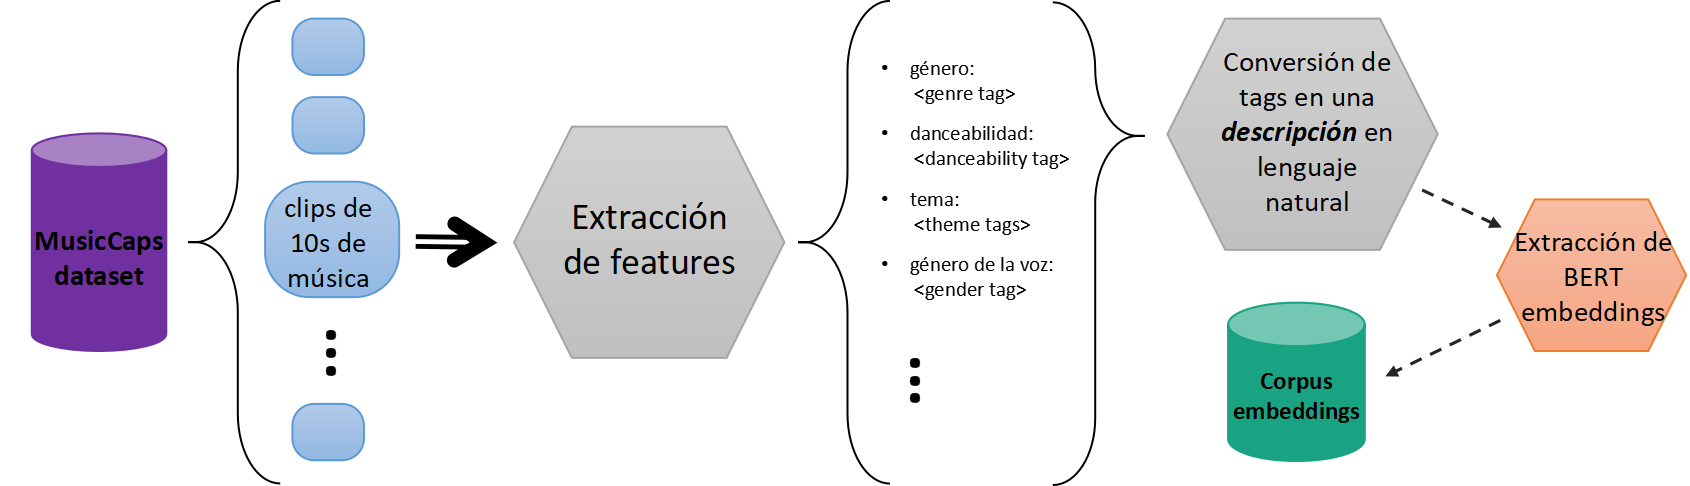
\includegraphics[width=\textwidth]{Graphics/corpus_embeddings.png}
	\caption{Diseño propuesto.} 
    \label{fig:corpus_embeddings}
\end{figure}

En el apartado de recuperación de información, el sistema consiste en recopilar la consulta del usuario, generar el vector de embedding con SBERT y encontrar las canciones más similares comparando el vector con el corpus de embeddings, utilizando similitud de coseno. En la imagen \ref{fig:sri_design} se observa el diseño del SRI. % TODO cite other BERT stuff that does this

\begin{figure}[h!]
	\centering
	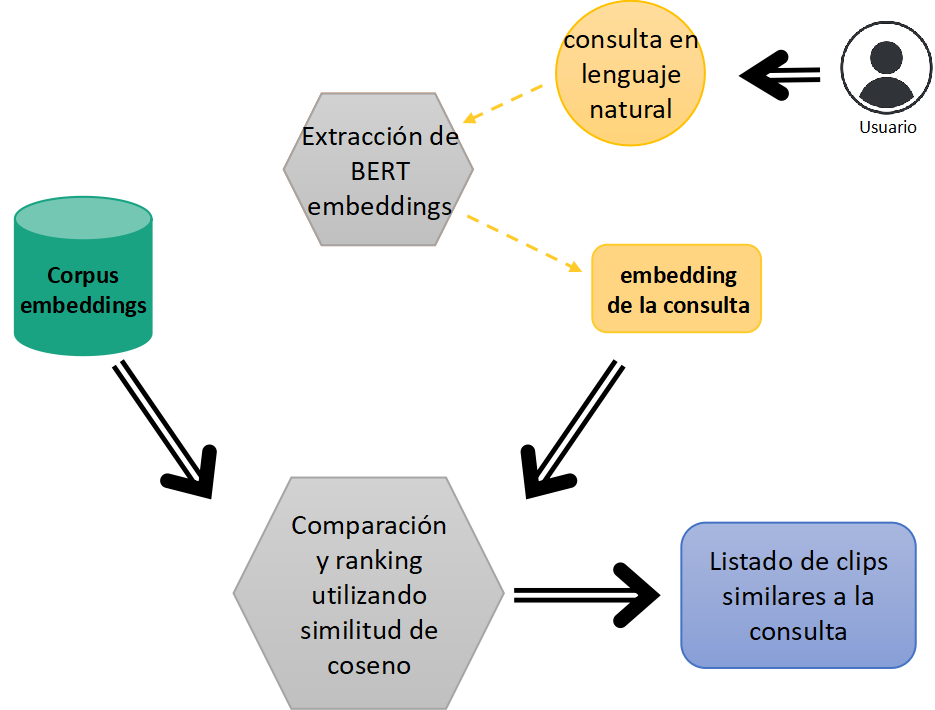
\includegraphics[width=0.6\textwidth]{Graphics/SRI.png}
	\caption{Sistema de recuperación utilizando \textit{Sentence BERT embeddings}.} 
    \label{fig:sri_design}
\end{figure}

\section{Dataset}
\label{sec:dataset}

Para establecer un baseline de la eficacia del prototipo a implementar es necesario evaluarlo con las métricas usuales en SRI y preferentemente en el mismo conjunto de datos que otros trabajos en el tema. 

\textit{Contrastive Audio-Language Learning for Music} \cite{Manco2022ContrastiveAL} entrenaron y evaluaron su modelo de recuperación en un \textit{dataset} de 250 mil pares (audio, texto) creado a partir de una biblioteca de música en producción. Pero no se encuentra disponible públicamente para utilizarlo y comparar justamente los resultados.

La evaluación de recuperación de música a partir de consultas textuales de \textit{MuLan: A Joint Embedding of Music Audio and Natural Language} \cite{Huang2022MuLanAJ} fue una colección patentada de 7,000 listas de reproducción curadas por expertos. Que tampoco fue encontrada públicamente.

Dado la idea mencionada en la sección \ref{subsec:music_captioning}, decidimos encontrar un \textit{dataset} de \textit{captioning}. Sin embargo la mayor parte de los datasets de captioning utilizados en la literatura son privados. Finalmente decidimos utilizar MusicCaps, que fue liberado públicamente en \cite{Agostinelli2023MusicLMGM}, una investigación apenas de este año. 

En \textit{HuggingFace} \cite{huggFaceMusicCaps} aparece una descripción del \textit{dataset}, el .csv y en \href{https://github.com/nateraw/download-musiccaps-dataset}{este link de github} hay un \textit{script} para descargar los clips de YouTube. MusicCaps contiene 5,521 clips de 10 segundos, extraídos de AudioSet \cite{Gemmeke2017AudioSA}. Por cuestiones de inaccesibilidad a la cantidad suficiente de internet, para esta investigación utilizamos un subconjunto de clips, lo que no causa ningún problema dado que no necesitamos una cantidad de datos específica con que entrenar. Cada clip contiene una lista de 'aspectos' en inglés y una descripción de texto libre escrita por músicos. Una lista de aspectos es, por ejemplo, "\textit{pop, tinny wide hi hats, mellow piano melody, high pitched female vocal melody, sustained pulsating synth lead}". Mientras que la descripción consta de varias oraciones sobre la música, por ejemplo, " \textit{A low sounding male voice is rapping over a fast paced drums playing a reggaeton beat along with a bass. Something like a guitar is playing the melody along. This recording is of poor audio-quality. In the background a laughter can be noticed. This song may be playing in a bar.} "

La escasez de datasets en MIR es un gran obstáculo en el desarrollo del campo. Se debe, en parte, a que a diferencia de otros tipos de multimedia, la música tiende a tener \textit{copyright} lo que impide crear conjuntos de datos con ejemplos representativos, que además sean lo suficientemente grandes para ser útiles en las arquitecturas de redes neuronales utilizadas en el presente aprender en el campo de texto, o imágenes, por ejemlo. Esto ha implicado que varias investigaciones recientes, incluyendo la nuestra, decidan apoyarse en las capacidades de transferencia de conocimiento que poseen los modelos de lenguaje, como fue explicado en la sección \ref{subsec:learning_lang_superv}, para tareas en MIR que incluyan trabajo con texto.
